\documentclass[11pt, leqno]{scrartcl}
\usepackage{polski}
\usepackage[polish]{babel}

\usepackage{graphicx, float, caption, subcaption}
\usepackage{tabularx, multirow, hyperref, enumitem}
\usepackage{listings, xcolor}
\usepackage{amsmath, amssymb}
%\usepackage{minted}

\hypersetup{
    colorlinks=true,
    linkcolor=black,
    urlcolor=black,
    citecolor=black
}

\definecolor{md-black}{rgb}{0.12, 0.12, 0.12}
\definecolor{md-teal}{rgb}{0.38, 0.79, 0.69}
\definecolor{md-mauve}{rgb}{0.76, 0.52, 0.75}
\definecolor{md-yellow}{rgb}{0.86, 0.86, 0.67}
\definecolor{md-green}{rgb}{0.13, 0.55, 0.13}
\definecolor{md-red}{rgb}{0.82, 0.10, 0.14}
\definecolor{md-purple}{rgb}{0.69, 0.33, 0.73}
\definecolor{md-orange}{rgb}{0.96, 0.42, 0.18}
\definecolor{md-gray}{rgb}{0.44, 0.46, 0.51}
\lstset{
    language=Python,
    basicstyle=\color{md-teal}\ttfamily,
    keywordstyle=\color{md-mauve},
    commentstyle=\color{md-green},
    stringstyle=\color{md-red},
    numbers=left,
    numberstyle=\small\color{md-gray}\ttfamily,
    stepnumber=1,
    numbersep=5pt,
    backgroundcolor=\color{md-black},
    showspaces=false,
    showstringspaces=false,
    showtabs=false,
    frame=none,
    tabsize=4,
    captionpos=b,
    breaklines=true,
    breakatwhitespace=false,
    escapeinside={\%*}{*)},
    numbersep=-10pt,
    morekeywords={as},
    classoffset=1,
    morekeywords={quad, quad_vec, trapz, simps, linregress,
        newton},
    keywordstyle=\color{md-yellow},
    classoffset=0
}

\graphicspath{{../images/}}

\title{Laboratorium 10 - Równania różniczkowe - spectral bias}
\author{Mateusz Podmokły - II rok Informatyka WI}
\date{28 maj 2024}

\begin{document}
    \maketitle
    \section{Treść zadania}
    \textbf{Zadanie 1.} Dane jest równanie różniczkowe zwyczajne
    \[
        \frac{du(x)}{dx}=cos(\omega x), \quad x \in \Omega
    \]
    gdzie: \\
    $x$, $\omega$, $u \in \mathbb{R}$, \\
    $x$ to położenie, \\
    $\Omega$ to dziedzina, na której rozwiązujemy równanie,
    $\Omega=\{x|-2\pi \leq x \leq 2\pi\}$, \\
    $u(x)$ to funkcja, której postaci szukamy.

    \subsection*{}
    Warunek początkowy zdefiniowany jest następująco:
    \[
        u(0)=0.
    \]
    Analityczna postać rozwiązania równania z warunkiem
    początkowym jest następująca:
    \[
        u(x)=\frac{sin(\omega x)}{\omega}
    \]
    Rozwiąż powyższe zagadnienie początkowe. Do rozwiązania
    użyj sieci neuronowych typu PINN (ang. Physics-informed Neural
    Network). \\
    Koszt rezydualny zdefiniowany jest następująco:
    \[
        \mathcal{L}_r(\theta)=\frac{1}{N}\sum_{i=1}^{N}
            \left| \left| \frac{d\hat{u}(x)}{dx}-cos(\omega x_i)
            \right| \right| ^2,
    \]
    gdzie $N$ jest liczbą punktów kolokacyjnych. \\
    Koszt związany z warunkiem początkowym przyjmuje postać:
    \[
        \mathcal{L}_{IC}(\theta)=||\hat{u}(0)-0||^2.
    \]
    Funkcja kosztu zdefiniowana jest następująco:
    \[
        \mathcal{L}(\theta)=\mathcal{L}_r(\theta)+
            \mathcal{L}_{IC}(\theta).
    \]
    Warstwa wejściowa sieci posiada 1 neuron, reprezentujący
    zmienną $x$. Warstwa wyjściowa także posiada 1 neuron,
    reprezentujący zmienną $\hat{u}(x)$. Uczenie trwa
    przez 50 000 kroków algorytmem Adam ze stałą uczenia równą
    0.001. Jako funkcję aktywacji przyjmij tangens hiperboliczny,
    $tanh(x)$.

    \subsection*{}
    Rozważ następujące przypadki:
    \begin{enumerate}
        \item Przypadek $\omega=1$. \\
            Ustal następujące wartości:
            \begin{itemize}[label=--]
                \item 2 warstwy ukryte, 16 neuronów w każdej
                    warstwie
                \item liczba punktów treningowych: 200
                \item liczba punktów testowych: 1000
            \end{itemize}
        \item Przypadek $\omega=15$. \\
            Ustal następujące wartości:
            \begin{itemize}[label=--]
                \item liczba punktów treningowych:
                    $200 \cdot 15=3000$
                \item liczba punktów testowych: 5000
            \end{itemize}
            Eksperymenty przeprowadź z trzema architekturami
            sieci:
            \begin{itemize}[label=--]
                \item 2 warstwy ukryte, 16 neuronów w każdej
                    warstwie
                \item 4 warstwy ukryte, 64 neurony w każdej
                    warstwie
                \item 5 warstw ukrytych, 128 neuronów w każdej
                    warstwie
            \end{itemize}
        \item Dla wybranej przez siebie sieci porównaj wynik
            z rozwiązaniem, w którym przyjęto, że szukane
            rozwiązanie ($ansatz$) ma postać:
            \[
                \hat{u}(x;\theta)=tanh(\omega x) \cdot
                    NN(x;\theta).
            \]
            Taka postać rozwiązania gwarantuje spełnienie warunku
            $\hat{u}=0$ bez wprowadzania składnika
            $\mathcal{L}_{IC}$ do funkcji kosztu.
        \item Porównaj pierwotny wynik z rozwiązaniem, w którym
        pierwszą warstwę ukrytą zainicjalizowano cechami Fouriera:
        \[
            \gamma (x)=[sin(2^0\pi x),cos(2^0\pi x),\dots,
                sin(2^{L-1}\pi x),cos(2^{L-1}\pi x)]
        \]
        Dobierz $L$ tak, aby nie zmieniać szerokości warstwy
        ukrytej.
    \end{enumerate}
    Dla każdego z powyższych przypadków stwórz następujące
    wykresy:
    \begin{itemize}[label=--]
        \item Wykres funkcji $u(x)$, tj. dokładnego rozwiązania
            oraz wykres funkcji $\hat{u}(x)$, tj. rozwiązania
            znalezionego przez sieć neuronową
        \item Wykres funkcji błędu.
    \end{itemize}
    Stwórz także wykres funkcji kosztu w zależności od liczby epok.

    \section{Specyfikacja użytego środowiska}
    Specyfikacja:
    \begin{itemize}
        \item Środowisko: Visual Studio Code,
        \item Język programowania: Python,
        \item System operacyjny: Microsoft Windows 11,
        \item Architektura systemu: x64.
    \end{itemize}

    \section{Rozwiązanie problemu}
    \subsection{Biblioteki}
    W realizacji rozwiązania wykorzystane zostały następujące
    biblioteki:
    \begin{lstlisting}
    import torch
    import torch.nn as nn
    import numpy as np
    import matplotlib.pyplot as plt
    \end{lstlisting}

    \subsection{Model sieci neuronowej}
    Do zaimplementowania modelu sztucznej sieci neuronowej PINN
    wykorzystałem bibliotekę \texttt{PyTorch}. Dane treningowe to
    równomiernie rozłożone punkty na przedziale $[-2\pi,2\pi]$
    zawierające krańce przedziału oraz warunek początkowy, czyli
    $x=0$. Natomiast jako dane testujące również wykorzystałem
    równomiernie rozłożone punkty na przedziale $[-2\pi,2\pi]$,
    jednak bez krańców przedziału, żeby uniknąć powtórzeń punktów.

    \section{Przedstawienie wyników}
    \subsection{Przypadek 1.}
    Parametry:
    \begin{itemize}
        \item $\omega =1$
        \item 2 warstwy ukryte, 16 neuronów w każdej warstwie
        \item 200 punktów treningowych
        \item 1000 punktów testowych
    \end{itemize}
    \begin{figure}[H]
        \centering
        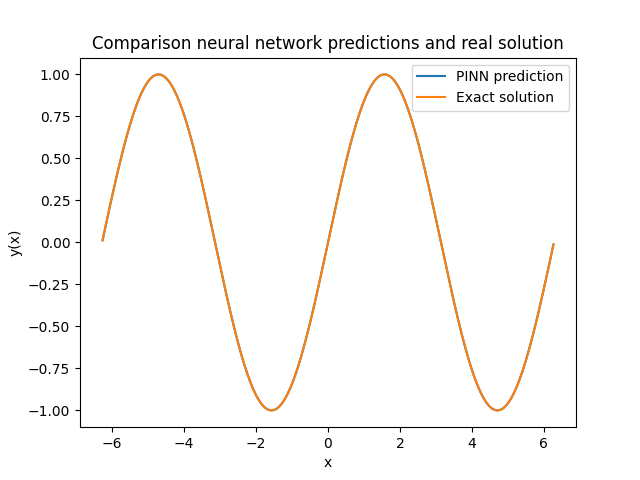
\includegraphics[width=0.7\linewidth]{nn_a_f.png}
        \caption{Dokładne rozwiązanie i rozwiązanie znalezione
            przez sieć, przypadek 1.}
    \end{figure}
    \begin{figure}[H]
        \centering
        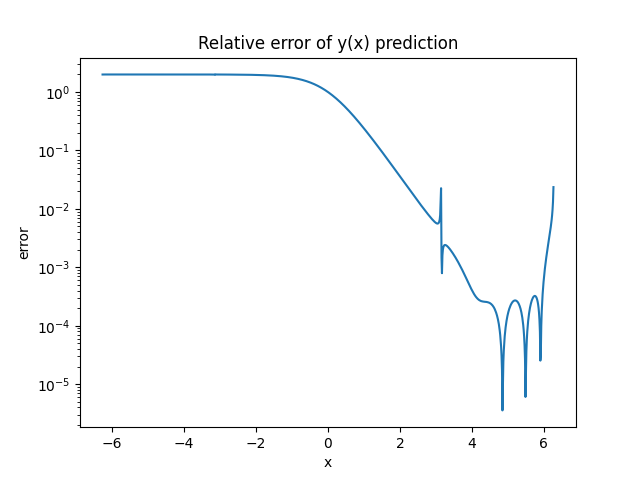
\includegraphics[width=0.7\linewidth]{nn_a_err.png}
        \caption{Błąd względny rozwiązania, przypadek 1.}
    \end{figure}
    \begin{figure}[H]
        \centering
        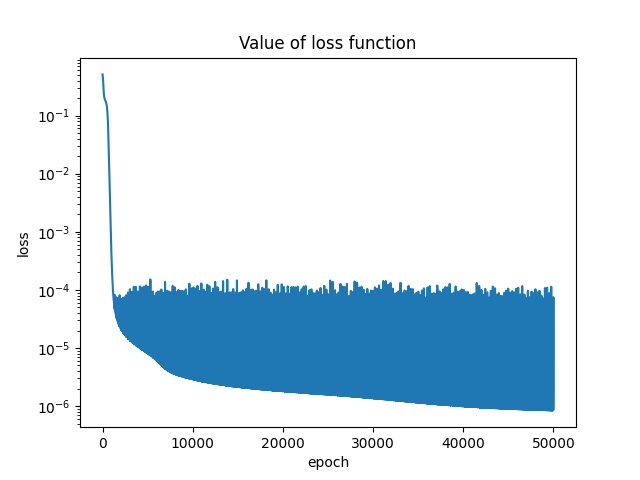
\includegraphics[width=0.7\linewidth]{nn_a_loss.png}
        \caption{Wartość funkcji kosztu w zależności od liczby epok,
            przypadek 1.}
    \end{figure}

    \subsection{Przypadek 2.}
    Parametry:
    \begin{itemize}
        \item $\omega =15$
        \item 2 warstwy ukryte, 16 neuronów w każdej warstwie
        \item 3000 punktów treningowych
        \item 5000 punktów testowych
    \end{itemize}
    \begin{figure}[H]
        \centering
        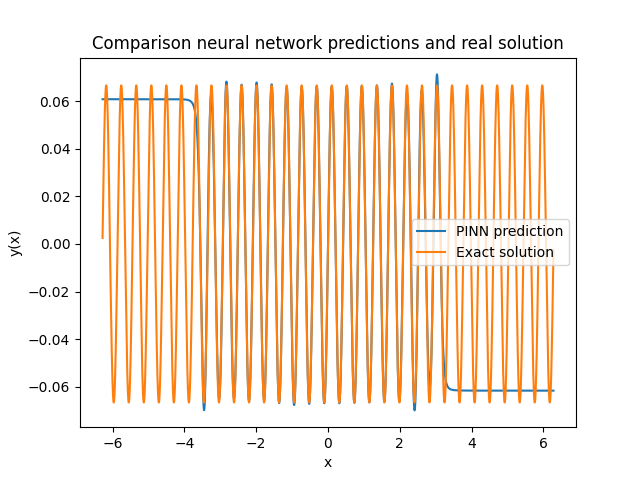
\includegraphics[width=0.7\linewidth]{nn_b1_f.png}
        \caption{Dokładne rozwiązanie i rozwiązanie znalezione
            przez sieć, przypadek 2.}
    \end{figure}
    \begin{figure}[H]
        \centering
        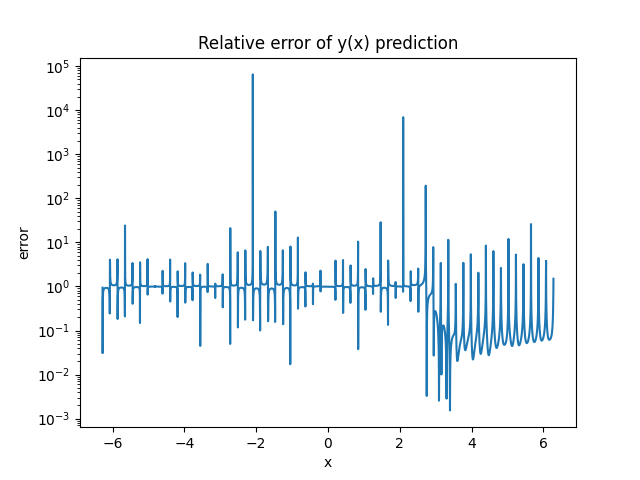
\includegraphics[width=0.7\linewidth]{nn_b1_err.png}
        \caption{Błąd względny rozwiązania, przypadek 2.}
    \end{figure}
    \begin{figure}[H]
        \centering
        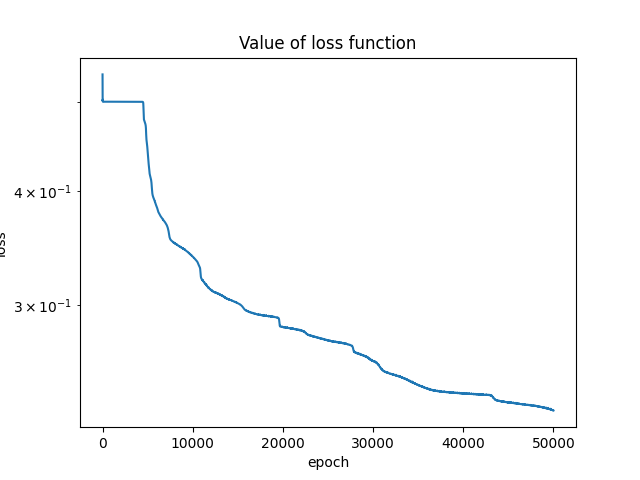
\includegraphics[width=0.7\linewidth]{nn_b1_loss.png}
        \caption{Wartość funkcji kosztu w zależności od liczby epok,
            przypadek 2.}
    \end{figure}

    \subsection{Przypadek 3.}
    Parametry:
    \begin{itemize}
        \item $\omega =15$
        \item 4 warstwy ukryte, 64 neurony w każdej warstwie
        \item 3000 punktów treningowych
        \item 5000 punktów testowych
    \end{itemize}
    \begin{figure}[H]
        \centering
        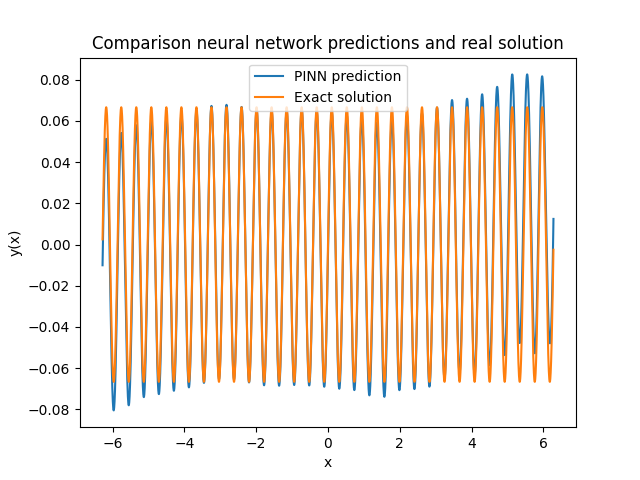
\includegraphics[width=0.7\linewidth]{nn_b2_f.png}
        \caption{Dokładne rozwiązanie i rozwiązanie znalezione
            przez sieć, przypadek 3.}
    \end{figure}
    \begin{figure}[H]
        \centering
        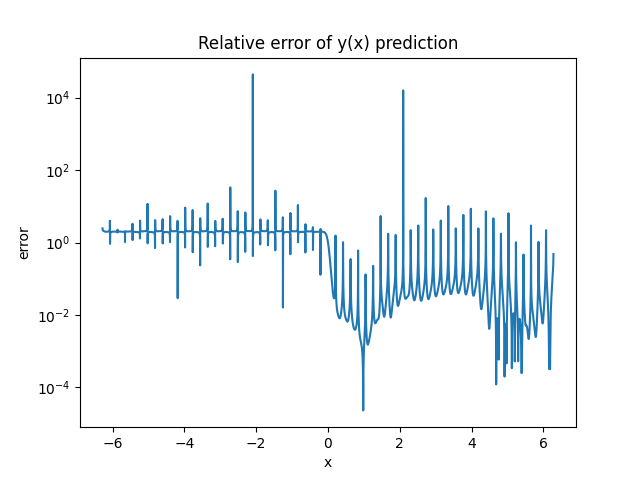
\includegraphics[width=0.7\linewidth]{nn_b2_err.png}
        \caption{Błąd względny rozwiązania, przypadek 3.}
    \end{figure}
    \begin{figure}[H]
        \centering
        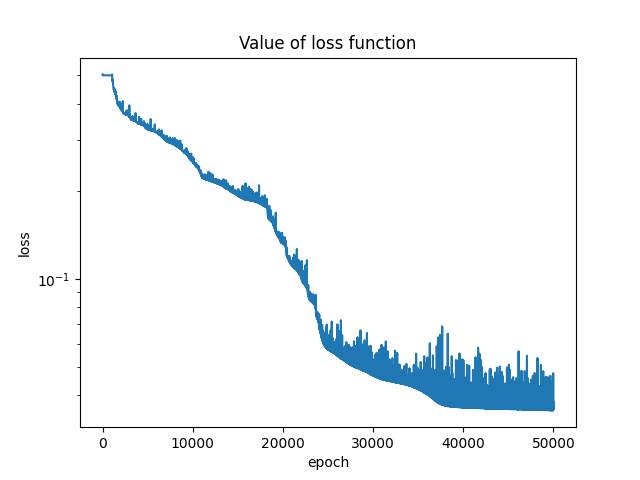
\includegraphics[width=0.7\linewidth]{nn_b2_loss.png}
        \caption{Wartość funkcji kosztu w zależności od liczby epok,
            przypadek 3.}
    \end{figure}

    \subsection{Przypadek 4.}
    Parametry:
    \begin{itemize}
        \item $\omega =15$
        \item 5 warstwy ukryte, 128 neuronów w każdej warstwie
        \item 3000 punktów treningowych
        \item 5000 punktów testowych
    \end{itemize}
    \begin{figure}[H]
        \centering
        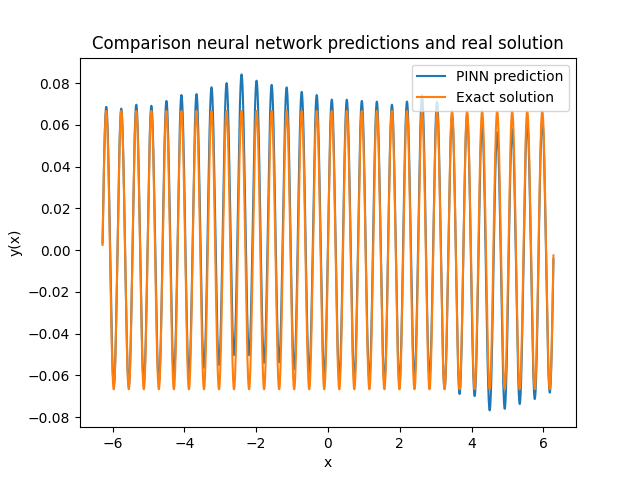
\includegraphics[width=0.7\linewidth]{nn_b3_f.png}
        \caption{Dokładne rozwiązanie i rozwiązanie znalezione
            przez sieć, przypadek 4.}
    \end{figure}
    \begin{figure}[H]
        \centering
        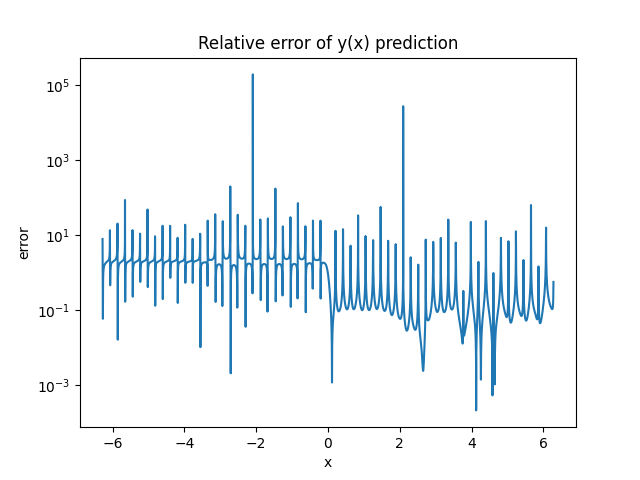
\includegraphics[width=0.7\linewidth]{nn_b3_err.png}
        \caption{Błąd względny rozwiązania, przypadek 4.}
    \end{figure}
    \begin{figure}[H]
        \centering
        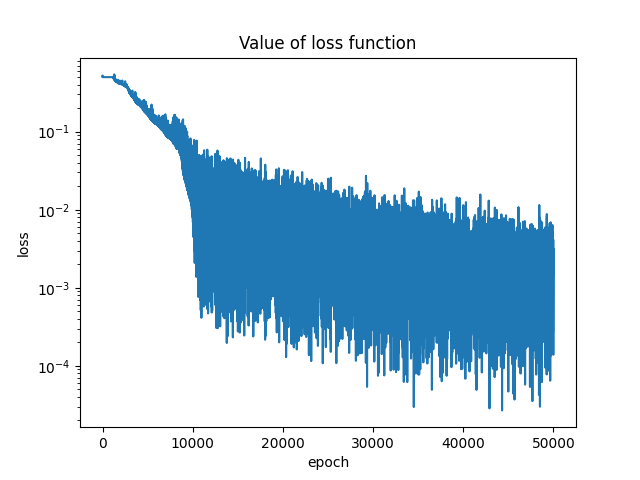
\includegraphics[width=0.7\linewidth]{nn_b3_loss.png}
        \caption{Wartość funkcji kosztu w zależności od liczby epok,
            przypadek 4.}
    \end{figure}

    \subsection{Przypadek 5.}
    Parametry:
    \begin{itemize}
        \item $\omega =15$
        \item 4 warstwy ukryte, 64 neuronów w każdej warstwie
        \item 3000 punktów treningowych
        \item 5000 punktów testowych
        \item szukane rozwiązanie ($ansatz$) ma postać:
            \[
                \hat{u}(x;\theta)=tanh(\omega x)\cdot NN(x;\theta)
            \]
    \end{itemize}

\end{document}
